\subsection{Repeated maps distinguish stable responses from map-sensitive effects}

Fidel's fixed-model response stayed positive under all twenty additional within-split nonzero cyclic shifts. Mean $\Delta$ MSE was 0.047600, the empirical 2.5th--97.5th percentile range was [0.032916,0.064487], and mean map-wise control-denominator SAG was 20.65\%. Positive-map counts for GPT-2, MiniLM and FinBERT were 0/20, 3/20 and 3/20 on FNSPID, and 2/20, 6/20 and 8/20 on EPA-Air. EPA-Air's effect direction thus depended on the map with model states and targets held fixed; Table~\ref{tab:maps} summarizes all seven cells.

Figure~\ref{fig:map_sensitivity} shows intervention-map sensitivity at the selected aligned states, separately from variation across entities or fitted models. Although aligned histories remained timestamp-restricted, offline shifts could assign later-dated donors; Supplementary Section~\ref{sec:map_conditioning} reports their timing fractions and denominators.

\begin{figure}[!htbp]
\centering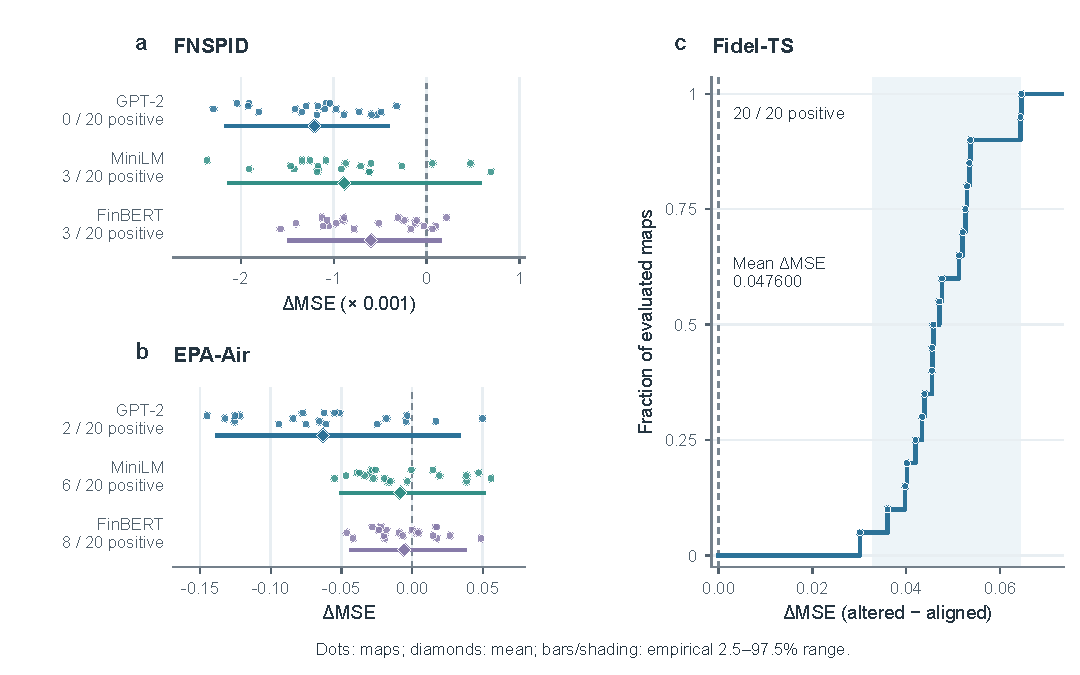
\includegraphics[width=\textwidth]{fig9_map_sensitivity}
\caption{Variation of fixed-model loss effects across the saved nonzero cyclic-shift maps. All 140 altered-minus-aligned MSE effects are retained: three encoder cells on FNSPID, three on EPA-Air and one shared-weather cell on Fidel. Each cell uses twenty maps of the same selected aligned state. (a,b) Encoder-specific effects are shown as strips. (c) Fidel effects are ordered by their empirical cumulative fraction. Zero separates greater altered-input loss from improvement. Bars and shading show saved 2.5th--97.5th percentiles over twenty maps, rather than sampling confidence intervals. Dataset-specific scales reflect different effect magnitudes. The numeric summaries appear in Table~\ref{tab:maps}.}
\label{fig:map_sensitivity}
\end{figure}

